\documentclass[12pt]{article}
\usepackage[lecture]{preamble}

%%%%%%%%%%%%%%%%%%%%%%%%%%%%%%%%%%%%%%%%%%%%%%%%%%%%%%%%%%%%%%%%%
%          Code Syntax Highlighting
%%%%%%%%%%%%%%%%%%%%%%%%%%%%%%%%%%%%%%%%%%%%%%%%%%%%%%%%%%%%%%%%%
\usepackage{fullpage}
\usepackage{listings}
\usepackage{color}
\usepackage{multirow}
\definecolor{mygreen}{rgb}{0,0.6,0}
\definecolor{mygray}{rgb}{0.5,0.5,0.5}
\definecolor{mymauve}{rgb}{0.58,0,0.82}
\lstset{
%   backgroundcolor=\color{},   % choose the background color
  basicstyle=\ttfamily,        % size of fonts used for the code
  breaklines=true,                 % automatic line breaking only at whitespace
  captionpos=b,                    % sets the caption-position to bottom
  commentstyle=\color{mygreen},    % comment style
  escapeinside={\%*}{*},          % if you want to add LaTeX within your code
  keywordstyle={\bfseries \color{blue}},       % keyword style
  stringstyle=\color{mymauve},     % string literal style
  language=C,
  numbers=none % Remove line numbers
}
% End

% package for images
\usepackage{graphicx}
\graphicspath{ {./images/} }




\begin{document}
%%%%%%%%%%%%%%%%%%%%%%%%%%%%%%%%%%%%%%%%%%%%%%%%%%%%%%%%%%%%%%%%%
%          Lecture 1: Into, Number Rep
%%%%%%%%%%%%%%%%%%%%%%%%%%%%%%%%%%%%%%%%%%%%%%%%%%%%%%%%%%%%%%%%%
\lecture[06/20/2023]{Intro, Number Rep}
The value of the \emph{i}th digit \emph{d} in any number base is $d \times \text{Base}^i$ where \emph{i} starts 0 and increases from right to left.

\subsection*{Signed Magnitude}
Similar to unsigned numbers but the most significant bit (first bit) represents if the number is positive or negative, this bit is called the \emph{sign bit}.

The issue with this representation is that there are two representations for the number 0, and operations are slow since there is additional work required to handel the sign bit.
\subsection*{Two's Complement}
The convention to represent signed numbers is called \textbf{Two's Complement}. The left most bit is the sign bit, and $1111 \; ... \; 1111_{\text{two}}$ is the most negative number. The advantage twos complement has over \emph{sign and magnitude} representation is that there is only one zero.

\subsubsection*{Negation Shortcut}
Simply flip bits, then add 1 to the result.
This reason this shortcut works is because the sum of a number and its inverted representation must be $1111 \; ... \; 1111_{\text{two}}$ \emph{(there is no carries)}.

Now since $x + \overline{x} = -1 $, we have $\overline{x} + 1 = -x$

\subsubsection*{Sign Extension Shortcut}
\begin{itemize}
    \item for positive 16 $\rightarrow$ 32 bit binary numbers, just add 16 zeros in the most significant bit
    \item For negative 16 $\rightarrow$ 32 bit binary numbers, copy the sign bit (which is 1) 16 times, placing it on the left of the number.
\end{itemize}

This works because positive numbers have an infinite number of leading zeros and negative numbers have an infinite number of leading ones.

\subsection*{One's Complement}
A representation in which the negative of a none's complement is found by inverting each bit. So now $11\dots110_{\text{two}}$ is equal to -1. This representation is similar to twos complement but has two 0s
\subsection*{Biased Notation}
A notation that represents the most negative value by $00 \ldots000_{\text{two}}$ and the most positive value by $11 \ldots 111_{\text{two}}$, with zero typically having the value $10 \ldots000_{\text{two}}$, thereby biasing the number such that the number plus the bias has a nonnegative representation.

In simpler words, bias notation is like unsigned representation but has a shift (a bias), shifting the range of values on the unsigned number line to the left, allowing representation of negative numbers.

With this new system, to interpret a binary string in bias notation, we evaluate the number as if it was unsigned, then add the bias (the bias is usually negative). Note we do this because we shift the numbers to the left by a bias.

\begin{example}[Interpreting a Stored Binary]
    Assume we have a $-127$ bias with an 8-bit number.

    To read $0b0000 \; 1001$, we treat it as if it was unsigned, which gives us 9. Then we add the bias to get our value $-118$:

    $9 + (-127) = -118$
\end{example}

To store a decimal number as a binary string in bias notation, we first subtract the bias (bias is negative so basically add) then store the resulting number as an unsigned binary.

\begin{lemma}
    Subtracting a bias will never give us a negative number.

    This is because the range of numbers is from $[-B, \;  2^n - 1 - B]$, where B is the magnitude of the bias. So a number $x$, will always be greater than or equal to $-B$, and obviously $x - (-B) \ge 0$.
\end{lemma}


\section*{Questions}
\begin{itemize}
    \item is right shift and left shift division and multiplication by 2 respectively?
\end{itemize}
%%%%%%%%%%%%%%%%%%%%%%%%%%%%%%%%%%%%%%%%%%%%%%%%%%%%%%%%%%%%%%%%%
%          Lecture 2: C Basics
%%%%%%%%%%%%%%%%%%%%%%%%%%%%%%%%%%%%%%%%%%%%%%%%%%%%%%%%%%%%%%%%%
\lecture[06/21/2023]{C Basics}
\section*{Chapter 0: Introduction}

The arguments to functions are passed by copying the value of the argument, and it is impossible for the called function to change the actual argument in the caller. When desired to achieve "call by reference," a pointer may be passed explicitly, and the function may change the object to which the pointer points.

Array name are passed as the location of the array origin, so array arguments are effectively call by reference.

C is not a strongly-typed language. It is relatively permissive about data conversion, although it will not automatically convert data types with the wild abandon of PL/I




\section*{Chapter 2: Types, Operators, and Expressions}

A \textbf{string constant} is a sequence of zero or more characters surrounded by double quotes. Underneath, a string is an array whos elements are single characters. The compiler automatically places the null character \lstinline|\0| at the end of each string, so the program can conveniently find the end.

\subsubsection*{Bitwise Operations}
In C, a leading 0 on an int constant implies \emph{\textbf{octal}}. A leading \lstinline|0x| indicates \emph{\textbf{hexa-decimal}}.

The bitwise AND operator \lstinline|&| is used to turn off bits.

The bitwise OR operator \lstinline||| is used to turn on bits.

The one's operator \lstinline|~| (one's complement) is used to flip bits.



\subsection{Memory Model Review}
Memory works very similar to an array. You can think of most version of memory you work with conceptually to be one very long array,

\subsubsection{The Stack}
The stack is memeory that is automatically allocated and freed by the system, and grows from top-down.
\textbf{What is the stack used for?}
\begin{itemize}
    \item Anything considered "Temporary"
    \item This includes: local variables, local constants, arguments to functions, local information about a function call.
\end{itemize}

\textbf{Stack Frames, function calls}
\begin{itemize}
    \item Everyime a function is called, a new "stack frame" is allocated on the stack
    \item Stack Frame Includes:
          \begin{itemize}
              \item return "instruction" address (who called me?), arguments, and space for other local variables
          \end{itemize}
    \item When function ends, stack frame is tossed off the stack; automatically frees memory for future stack frames.
\end{itemize}


\subsubsection{The Heap}





\section*{Questions}
\begin{itemize}
    \item What is an example of local information about a function call?
\end{itemize}


%%%%%%%%%%%%%%%%%%%%%%%%%%%%%%%%%%%%%%%%%%%%%%%%%%%%%%%%%%%%%%%%%
%          Lecture 3: C Pointers, Arrays, Memory Management
%%%%%%%%%%%%%%%%%%%%%%%%%%%%%%%%%%%%%%%%%%%%%%%%%%%%%%%%%%%%%%%%%
\lecture[06/22/23]{C Pointers, Arrays, Memory Management}

% TODO DELETE Section
\lecture[06/27/23]{C Memory}
Stack grows down, i.e, starts af FF and decreases.

The stack memory is destroyed as you return from functions

The heap memory does not, you are responsible for destorying (freeing) the memory when you don't need it anymore.


\section*{Chapter 5: Pointers and Arrays}
\begin{definition}[Pointer]
    A pointer is a variable that contains the address of another variable. The convention to naming pointer variables is the prefix them with \lstinline|p_<name>|.

    An pointer that points to an \lstinline|int| is declared as follows:

    \lstinline{int *p_x;}

    It says that the combination of \lstinline|*p_x| is an \lstinline|int|, that is, if the derefencing operator is used on \lstinline|p_x|, it is equivalent to a variable of type \lstinline|int|.
\end{definition}


\begin{itemize}
    \item The unary operator \lstinline|&| gives the \emph{address} of an object.
    \item The dereference operator \lstinline|*| used in the context as an operand to an address, access that address to fetch the contents to which it points to.
\end{itemize}






\subsection*{Pointers and Syntax}
\begin{itemize}
    \item pointers can occur on the left side of assignments. That is \lstinline{p_x} points to \lstinline{x}, then \\ \lstinline{*p_x = 1} sets \lstinline{x} to 1.
    \item Normally a pointer can point to only one type, however, \lstinline{void *} is a type that can point to anything. (use sparingly)
\end{itemize}

\subsection*{Arrays}
Arrays and pointers have a strong relationship. The name of an array is actually an address location to the zeroth element in the collection. \newline
So saying \lstinline{p_arr = arr} is equivalent to saying \lstinline{p_arr = &arr[0]}

Moreover, indexing into an array is actually using pointer arithmetic under the hood. For example: doing \lstinline{arr[3]} is equivalent to \lstinline{*(a + 3)}.

\subsubsection*{Address Arithmetic}
The only difference between an array name and a pointer is that a pointer is a variable, but an array name is a \textbf{constant}. Constructions like \lstinline{a = p_arr} or \lstinline{a++} or \lstinline{p = &a} are illegal.


\subsubsection*{Memory Organization}
Memory is just a large, single-dimensional array with the, that is byte-addressable, where the address acting as the index to that array. 8 bits = 1 byte, and 4 bytes = 1 word.



\textbf{Type Sizes:} Assume we are working with a 32-bit system.
\begin{itemize}
    \item \lstinline{int} occupy 4 bytes, aka 32 bits.
    \item \lstinline{char} occupy 1 byte
    \item \emph{pointers} occupy 4 bytes. This is because memory address are 32 bits long in a 32-bit system (why?), therefore the pointer values, the address that the pointer points to, are also 32 bits long.
\end{itemize}
\begin{definition}[Endianness Systems]
    Endianness affects how a group of bytes are stored and read in memory.

    \textbf{Little-Endian:} In a little-endian system, memory is stored with the most significant byte at the height address.

    \textbf{Big-Endian:} In a big-endian system, memory is stored with the most significant byte at the lowest address.
\end{definition}

\begin{example}
    For the program below assume, the memory is drawn as such in little endian system.

    \begin{lstlisting}
        int main() {
            int x[2]; // address of x is: 0x1000 0000
            x[0] = -2, x[1] = 44513;
            char y[] = "ADEL"; // address of y is: 0x1000 0010
            char *c y;
        }
    \end{lstlisting}

    The corresponding memory model is as follows

    \begin{center}
        \begin{tabular}{|c|>{\centering\arraybackslash}p{2cm}|>{\centering\arraybackslash}p{2cm}|>{\centering\arraybackslash}p{2cm}|>{\centering\arraybackslash}p{2cm}|}
            \hline
            \textbf{Address} & \textbf{Byte 0} & \textbf{Byte 1} & \textbf{Byte 2} & \textbf{Byte 3} \\
            \hline
            0x1000 0000      & 0xFE            & 0xFF            & 0xFF            & 0xFF            \\
            \hline
            0x1000 0004      & 0xE1            & 0xAD            & 0x00            & 0x00            \\
            \hline
            0x1000 0008      & -               & -               & -               & -               \\
            \hline
            0x1000 000C      & -               & -               & -               & -               \\
            \hline
            0x1000 0010      & 0x41            & 0x44            & 0x45            & 0x4C            \\
            \hline
            0x1000 0014      & 0x00            & -               & -               & -               \\
            \hline
            0x1000 0018      & 0x10            & 0x00            & 0x00            & 0x10            \\
            \hline
        \end{tabular}
    \end{center}

    \textbf{Note:} While \lstinline{ints} get stored in reverse, character arrays or strings are stored in increasing memory addresses.


\end{example}


\begin{itemize}
    \item type declaration tells compiler how many bytes to fetch on each access through pointer.
    \item
\end{itemize}

\subsubsection*{Dynamic Allocation}
\begin{itemize}
    \item malloc: memory Allocation
    \item calloc: cleared allocation
    \item realloc: re-allocation
\end{itemize}


68 6c 70 74 78 7c 80 84 88 8c 90





\section*{Questions}
\begin{itemize}
    \item is there double pointers, a pointer that points to another pointer? \textbf{Yes, you write a function to increment a pointer. Here it will accept a double point as an argument}
    \item Is there null in C? Can you initialize a pointer to be null? \textbf{Yes, C has a null keyword, NULL}
    \item It is said that the difference between arrays and pointers is that array names is a constant, not a variable. Can you have a pointer to a constant? Why is \lstinline{p = &arr} illegal?

\end{itemize}



\lecture[06/27/23]{Floating Point}

Just as we can show decimal numbers in scientific notation, we can also show binary numbers in scientific notation:
$$
    1.0_{\text{two}} \times 2^{-1}
$$

To keep a number in normalized form, we need a base that allows us to shift the binary point left or right to have on nonzero digit to the left of the decimal point. Only base 2 fulfills this since multiplication by 2 is a left shit and division is a right shift.


\begin{definition}[Floating point]
    Computer arithmetic that represents numbers in which the binary point is not fixed, i.e., it floats.
    The floating-point representation is as such:\\

    \begin{center}
        \begin{tabular}{|*{32}{c}}
            \hline
            31                      & 30                            &                                         &  &  &  &  &  &  & 23 & 22 &  &  &  &  &  &  &  &  &  &  &  &  & \multicolumn{1}{c|}{0} \\ \hline

            \multicolumn{1}{|c|}{s} & \multicolumn{9}{c|}{exponent} & \multicolumn{14}{c|}{fraction/mantissa}                                                                                          \\ \hline
        \end{tabular}
    \end{center}

    The scientific notation in binary form of the float is a singly nonzero digit to the left of the binary point (\textbf{normalized form}) as such:

    $$
        1.\underbrace{xxxxxxxxx_{\text{two}}}_{\color{orange}{\text{mantissa/significand}}} \times 2^{\text{yyyy} \rightarrow \color{blue}{\text{exponent}}}
    $$
    Where $1.xxxxxxxxx$ is the significand ($0 < S < 1$), and $yyyy$ is called the exponent.

    To pack more numbers in the significand, IEEE 754 makes the leading 1-bit of a normalized binary numbers implicit. So now, the mantissa is $1 + \text{23-bit significand field}$. Therefore, the simple RISC-V floating number as such:

    $$
        (-1)^S \times (1 + F) \times 2^E
    $$
    Where $S$ is the sign of the floating-point number, $F$ involves the value in the fraction field, generally a number between 0 and 1, also called the \emph{mantissa}. And $E$ comes from the exponent field.

    Note however, float comparisons are hard with this form. The most negative exponent is all 1s, and $1_\text{ten}$ is a single 1 bit in the least significant bit. The negative number looks larger. Therefore we introduce bias notation to shift the numbers where now the most negative number is $00 \dots 00_{\text{two}}$ and the most positive as $11 \dots 11_{\text{two}}$. IEEE 754 uses a bias of 127 for single precision, and 1023 for double precision.

    Biased exponent means that the value represented by a floating-point number is really:


    $$
        (-1)^S \times (1 + F) \times 2^{E - \text{Bias}}
    $$
\end{definition}


\begin{example}
    What is the decimal equivalent of the following IEE 754 single-precision binary floating point number?
    \begin{center}
        \begin{tabular}{|*{32}{c}}
            \hline
            31                      & 30                             &                                         &  &  &  &  &  &  & 23 & 22 &  &  &  &  &  &  &  &  &  &  &  &  & \multicolumn{1}{c|}{0} \\ \hline

            \multicolumn{1}{|c|}{1} & \multicolumn{9}{c|}{1000 0001} & \multicolumn{14}{c|}{111 0000 ... 0000}                                                                                          \\ \hline
        \end{tabular}
    \end{center}

    \begin{align}
         & = (-1)^1 \times 1.111 \times 2^{129 - 127}                                          \\
         & = -1 \times 1.111 \times 2^{2}                                                      \\
         & = -1 \times 111.1                          &  & \text{shift the decimal point by 2} \\
         & = -1 \times (4 + 2 + 1 + \frac{1}{2})                                               \\
         & =  -7.5
    \end{align}
\end{example}

\subsection*{Step Size}
Because we have a fixed \# of bits, we cannot represent all numbers. \textbf{Step size} is the spacing between consecutive floats with a given exponent.

What we really are asking for is what is the next representable number after y? before y?

The next step size to why is just adding y to the smallest bit in the significand times the same exponent.
$$
    y + ((0.0\dots001) \times 2^{(E - Bias)})
$$

Note we multiply by the same exponent because y decimal was shifted, so we also need to shift the smallest bit decimal to the same position.

\emph{Note:} the bigger the exponent, the bigger the step size since it's shifted more.
And the smaller the exponent, the smaller the step size


\subsection*{Representing Zero}
Note: Zero has no normalized representation (there is always an implicit 1 in the significand)



%%%%%%%%%%%%%%%%%%%%%%%%%%%%%%%%%%%%%%%%%%%%%%%%%%%%%%%%%%%%%%%%%
%          Lecture 6: Risc-V Intro
%%%%%%%%%%%%%%%%%%%%%%%%%%%%%%%%%%%%%%%%%%%%%%%%%%%%%%%%%%%%%%%%%
\lecture[06/28/23]{Risc-V Intro}The operands of arithmetic instructions are restricted, in that they must be from a limited number of special locations built directly in hardware called \emph{registers}.
\begin{definition}[Registers]
    Registers are primitives used in hardware design, often thought of as the "bricks of computer construction". The size of a register in RISC-V architecture is 32 bits, aka 1 word.

    There is a limited number of registers, 32 registers. The reason for the limit of 32 registers is because of the underlying design principles of hardware; \textbf{smaller is faster.} Accessing registers takes less time and uses much less energy than accessing memory.


\end{definition}

In code, we usually have more complex data structures such as arrays. These data structures usually contain more data elements than there are registers. How can a computer represent and access such large structures? They are kept in memory and accessed via instructions that transfer data between memory and registers. Such instructions are called \textbf{data transfer instructions.}

It is the computer job to associate program variables with registers. Usually a program contains many more variables than computer registers. The compiler tries to keep the most frequently used variables in registers and places the rest in memory, data transfer instructions to between registers and memory. This process is called \emph{spilling registers}.


%%%%%%%%%%%%%%%%%%%%%%%%%%%%%%%%%%%%%%%%%%%%%%%%%%%%%%%%%%%%%%%%%
%          Lecture 7: RISC-V Procedures
%%%%%%%%%%%%%%%%%%%%%%%%%%%%%%%%%%%%%%%%%%%%%%%%%%%%%%%%%%%%%%%%%
\lecture[06/29/23]{RISC-V Procedures}
\subsection*{Calling Convention}

Saved Registers:
\begin{itemize}
    \item s0-s11 ra
    \item should not be modified by functions (can be used, but must be restored).
\end{itemize}

Temporary Registers:
\begin{itemize}
    \item {\color{red} TODO}
\end{itemize}


Stack


%%%%%%%%%%%%%%%%%%%%%%%%%%%%%%%%%%%%%%%%%%%%%%%%%%%%%%%%%%%%%%%%%
%          Lecture 8: RISC-V Instruction Format
%%%%%%%%%%%%%%%%%%%%%%%%%%%%%%%%%%%%%%%%%%%%%%%%%%%%%%%%%%%%%%%%%
\lecture[07/05/23]{RISC-V Instruction Format}
Instructions are kept in the computer as a series of high and low (1s and 0s) electronic signals and may be represented as numbers. Placing these numbers side by side forms the instruction. The numeric version of instructions is called \textbf{machine language}, and a sequence of such instructions is called \emph{machine code}.

Instructions in the numeric version are split up into \textbf{fields}, which are given names to make them easier to discuss. Here is the meaning of each name of the fields in RISC-V instructions:
\begin{itemize}
    \item \emph{\textbf{opcode:}} Instruction identifier. The field that denotes the operation and format of an instruction, and is always the last 7 bits in all instruction formats.
    \item \emph{rd:} The register destination operand. It gets the result of the operation.
    \item \emph{funct3:} An additional opcode field.
    \item \emph{rs1:} The first register source operand.
    \item \emph{rs2:} The second register source operand.
    \item \emph{funct7:} An additional opcode field.
\end{itemize}

Different instructions require different fields sizes. For example, \lstinline{add} requires 3 registers, \lstinline{addi} requires 2 registers and 1 immediate. If rs2 took the value of the immediate, the maximum size it could hold is $2^5 - 1$ (31 which is pretty small) since rs2 is 5 bits long. Since RISC-V designers decided to keep all instructions the same length (32 bits), this requires distinct instruction formats for different kinds of instructions.

The formats are distinguished by the values in the opcode field (check reference sheet to see the different types of formats).

\subsection*{R-Type}
Designed for instructions with 3 registers and no immediate.

Since each register is identified by it's number, we'd need 5 bits to encode 32 different values ($2^5 = 32$).


\subsection*{I-Type}
Designed for instructions with 2 registers (rs1 and rd) and 1 immediate.
Some instructions that use I-Types include arithmetic operations with immedates and load instruction.

In the R-Type, there is no funct7 field, instead, that space is used by the immediate the be able to get larger constants (12 bits long immediate)

The immediate field is in unsigned representation, so the range of values is [-2048, 2047] [$-2^{11}, 2^{11} - 1$]

\subsection*{I*-Type}
Used for shifting with immediates (slli, srli, srai) where the immediate field is reduced to 5 bits long. This is because in shifting a 32-bit number, you never need to shift more than 32 times.

\subsection*{S-Type}
S for \textbf{store instructions}. Designed for instructions with 2 source registers and an immediate.


\subsection*{U-Type}
Used for \lstinline{lui} (\emph{load upper immediate}) and \lstinline{auipc} (\emph{add upper immediate to program counter}) instructions.

These two instructions are used in two pseudoinstructions:
\begin{itemize}
    \item \lstinline{li}: load immediate
    \item \lstinline{la}: load address
\end{itemize}

\begin{example}[\lstinline{li} with Large Immediate]
    consider this instruction:
    \begin{lstlisting}
        li t0 0x12345678
    \end{lstlisting}
    We cannot just translate this instruction to: \lstinline{addi t0 x0 0x12345678} since the immediate size of \lstinline{addi} is 5 bits long. Assuming that lui has an immediate size of 20 bits (which it does), the solution then is to do this:

    \begin{lstlisting}
        lui to 0x12345 // 20 bit long immediate (5 * 4)
        addi t0 t0 0x678 // 12 bit immediate (fits in addi immediate field.)
    \end{lstlisting}
    * \emph{Note there is a corner case when the immediate in an li instructions has FFF in the 3 right most bits, since addi with an immediate of FFF subtracts $-1$. }
\end{example}

\subsection*{B-Type}
B for branch instructions. Recall, labels don't actually exist. When translating RISC-V to machine language, we need to convert all labels into explicit references to a particular line of code. Since we want to be able to move around code blocks in memory, we prefer to use \textbf{\emph{relative addressing}} instead of absolute addresses.

Therefore, when writing code using labels, we first convert the label into an \emph{offset}, which specifies how many bytes off from the current location (\lstinline{PC} - program counter) we would need to jump to get to that label.

\begin{example}[Converting Labels to Offsets]
    Consider the following code
    \begin{lstlisting}
        beq x0, x0, target // + 2 instructions = 8 bytes, so offset = 8
        addi x0, x0, 100
        target: addi x0, x0, 100 
        j target           // - 1 instruction = -4 bytes, so offset = -4
        li t0 0x5F3759DF
        beq t0, t0, target // -4 instructions = -16 bytes, so offset = -16
    \end{lstlisting}
    \emph{* note li is a pseudoinstructions for 2 instructions}
\end{example}

\subsubsection*{Storing Offsets:}
Note all of the previous offsets were multiples of 4 since each instruction is 4 bytes of memory, so all offsets should be multiples of 4. Therefore, the last two bits off the offset are always going to be 0s. For optimization purposes, we don't store the lowest bit of an offset immediate, brining forth the assuming that the LSB an offset is 0.

In the instruction format, the immediate representing the offset is stored in a strange pattern:
\lstinline{imm[12 | 10:5]}  for bits 31 through 25 of the B-Type format, and \lstinline{imm[4:1 | 11]} for bits 11 thorough 7.
\begin{itemize}
    \item if we have the binary $\text{0b A BCDE FGHI JKLM}$ (where each letter was a bit), the first immediate field would store $\text{0b ACD EFGH}$.
    \item the second immediate field would store $\text{0b I JKLB}$. \emph{note bit M isn't stored}
\end{itemize}



\subsection*{J-Type}
J for jump instruction, \lstinline{jal}. This instruction uses only 1 destination register and an immediate example: \lstinline{jal ra label}, so we can use the U-type format to have a larger immediate, but the immediate is stored in a strange format, to simplify the underlying circuit.

The immediate is stored as: \lstinline{imm[20 | 10:1 | 11 | 19:2]}

For example: If we had the binary $\text{0xA BCDE FGHI JKLM NOPQ RSTU}$ (where each letter was a bit), the data would be stored as 0b $\text{AKLM NOPQ RSTJ BCDE FGHI}$



%%%%%%%%%%%%%%%%%%%%%%%%%%%%%%%%%%%%%%%%%%%%%%%%%%%%%%%%%%%%%%%%%
%          LECTURE 9: Compiler, Assembler, Linker, Loader
%%%%%%%%%%%%%%%%%%%%%%%%%%%%%%%%%%%%%%%%%%%%%%%%%%%%%%%%%%%%%%%%%
\lecture[07/06/23]{Compiler, Assembler, Linker, Loader: CALL}
\subsection*{Compiler}
The compiler transforms the C program into an \textbf{assembly language} program, a symbolic form of what the machine understands.

\begin{definition}[Assembly Language]
    a symbolic language that can be translated into binary machine language.
\end{definition}

\subsection*{Assembler}
The assembler converts \textbf{pseudoinstructions} into the machine language equivalent of the actual assembly language instruction. It also converts branches to faraway locations into a branch and a jump.
\begin{definition}[Pseudoinstructions]
    A common variation of assembly language instructions often treated as if it were an instruction in its own right.
\end{definition}
The primary task of an assembler is assembly into machine code. The assembler turns the assembly language program into an \emph{object file}, which is a combination of machine language instructions, data, and information needed to place instructions properly in memory.

To Produce binary version of each instruction into assembly language program, the assembler must determine the address corresponding to all labels. Assemblers keep track of labels used in branches and data transfer instruction in a \textbf{symbol table}.

\subsection*{Linker}
The linker produces an \textbf{executable file} that can be run on a computer.
The linker resolves all references, resolving all undefined labels, patching both internal and external references.

\subsection*{Loader}
A systems program that places an object programs n main memory is that it is ready to execute.


\lecture[07/10/23]{Combinational Logic, FSM}

\section*{A.2: Gates, and Logic Equations}
Blocks without memory are called \emph{combinational}; the output of a combinational block depends only on the current input.

In blocks with memory, the output can depend on both the current input and the value stored in memory, which is called the \emph{state} of the logic block.

\begin{definition}[Combinational Logic]
    A logic system whose blocks do not contain memory and hence compute the same output given the same input.
\end{definition}

Since combinational logic block contains no memory, it can be completely specified by defining the values of the outputs for each possible set of input values. Such a description is normally given as a \emph{truth table.} Truth tables can completely describe any combinational logic function; however; they grow in size quickly ($2^n$ entries for $n$ inputs) making them hard to understand.

\subsection*{Boolean Algebra}
Used to represent signals in logic circuits. One alternative to truth tables is to express the logic function with logic equations. In boolean algebra, all the variables have the values 0 or 1, and in typical formulations, there are three operators:

\begin{itemize}
    \item OR operator, written as $A + B$.
    \item AND operator, written as $A \cdot B$.
    \item unary NOT operator, written as $\overline{A}$
\end{itemize}

Any set of logic functions can be written as a series of equations with an output on the left-hand side of each equation and a formula consisting of variables and the three operators above on the right-hand side.

\subsection*{Gates}
A device that implements basic logic functions, such as AND or OR.

Since both AND and OR are commutative and associative, they can take in multiple inputs, with the output equal to the AND or OR of all the inputs.

Fact: all logic functions can be constructed with only a single gate type, if that gate is inverting. NOR and NAND gates are called \emph{universal}, since any logic function can be built using this one gate type.

\section*{A.3: Combinational Logic}
 {\color{red} TODO}


\section*{FSM: Finite State Machines}
 {\color{red} TODO}

\subsubsection*{Questions}
\begin{itemize}
    \item is the memory contained inside the logic block called the state? or is the output called the state?
    \item
\end{itemize}

%%%%%%%%%%%%%%%%%%%%%%%%%%%%%%%%%%%%%%%%%%%%%%%%%%%%%%%%%%%%%%%%%
%          Lecture 11: Synchronous Digital Systems
%%%%%%%%%%%%%%%%%%%%%%%%%%%%%%%%%%%%%%%%%%%%%%%%%%%%%%%%%%%%%%%%%
\lecture[07/11/23]{Synchronous Digital Systems}
Synchronous Digital Systems are made up of two basic types of circuits. Combinational Logic circuits, and state elements. \textbf{Combinational logic} circuits change based on their inputs after whatever propagation delay is associated with them. Their like a function.

\section*{State Elements}
\textbf{State elements,} on the other hand can \emph{remember} their inputs even after the inputs change. State elements change value based on a \emph{clock signal.}
\subsubsection*{Clock:}
\begin{itemize}
    \item Rising Edge: Time when the clock switches from 0 to 1
    \item Falling Edge: Time when the clock switches from 1 to 0.
    \item Clock Period: Time between rising edges.
    \item Clock Frequency: Number of rising edges per second.
\end{itemize}

Like logic gates, registers also have a delay associated with them before their output will reflect the input that was sampled at the rising edge of the clock. This is called \textbf{clk-to-q} delay ("Q" often indicates the output.) This is the time between the rising edge of the clock signal and the time the register's output reflect the input change.

\subsection*{Flip Flop}
A Flip Flop is a logic element that 'stores state'.
On the rising edge of the clock, the input is sampled and transferred to the output. At all other times, the input is ignored.

For circuits with multiple flip flops, the flip flop respond to the input at a single time instant when the click is at a rising edge.

\subsubsection*{Time Constraints}
Flip flop sometimes have what's called time constraints. ($t_{\text{setup}}$, $t_{\text{hold}}$) These are \textbf{not} delays, but referred to as constraints because they must be followed inorder for the circuit to work properly. Below is the definition of the timing constraints:

\textbf{setup time}: $t_{\text{setup}}$
\begin{itemize}
    \item This is the amount of time that the flip flop input needs to be stable \emph{\textbf{BEFORE}} the positive edge of the clock.
\end{itemize}


\textbf{hold time}: $t_{\text{hold}}$
\begin{itemize}
    \item the minimum amount of time that the flip-flop input needs to be stable \emph{\textbf{AFTER}} the positive edge of the clock.
\end{itemize}

\subsubsection*{Satisfying setup time constraint (minimum clock period)}
Note during a single clock period, there is a clk-to-q time delay, and some logic delay (assuming there is logic elements in the circuit), and finally a setup time constraint for the next rising edge. Therefore, we need to have a clock period to be long enough so that it could hold all of these timing constraints and delays.

$$t_{\text{clk-to-q}} + t_{\text{logic max}} + t_{\text{setup}} \le t_{\text{clk-period}}$$

\subsubsection*{Satisfying hold time constraint}
It is easy to see that for a circuit without a logic elements, the hold time for a flipflop should always be less than or equal to the clk-to-q.

However, when circuits contain logic elements, which have delays of their own, we'd need to hold time to be short enough so that it is less than the sum of the clk-to-q and the shortest logic delay path. Therefore, the inequality needed so that we don't violate the hold time constraint is as such:

$$
    t_{\text{clk-to-q}} + t_{\text{logic min}} \ge t_{\text{hold}}
$$


%%%%%%%%%%%%%%%%%%%%%%%%%%%%%%%%%%%%%%%%%%%%%%%%%%%%%%%%%%%%%%%%%
%          Lecture 12: Single Cycle Datapath
%%%%%%%%%%%%%%%%%%%%%%%%%%%%%%%%%%%%%%%%%%%%%%%%%%%%%%%%%%%%%%%%%

\lecture[07/12/23]{RISC-V Single Cycle Datapath}

For every implementation of instructions; the first two steps are identical, the other steps are dependent on the type of instruction.
\begin{enumerate}
    \item Send the \emph{program counter} (PC) to the memory that contains the code and fetch the instruction from that memory.
    \item Read one or two registers, using fields of the instruction to select the registers to read. For the \lstinline{lw} instruction, we need to read only one register, but most other instructions require reading two registers.
    \item execute the operation or calculate an address
    \item Access an operand in data memory (if necessary)
    \item Write the result into a register (if necessary)
\end{enumerate}

After these two steps, the actions required to complete the instruction depend on the instruction class (memory-reference, arithmetic-logical, or branches).

\begin{definition}[Control Unit]
    A \emph{control unit} has an instruction as an input, and  is used to determine how to set the control lines for the functional units and two of the multiplexors.
\end{definition}


\subsection*{Building a Datapath}
To execute any instruction, we must start by fetching the instruction from memory (code section of the memory?)
To prepare for executing the next instruction, we must also incremenet the PC so that it points at the next instruction, 4 bytes later.

The processor's 32 general-purpose registers are stored in a structure called a \textbf{register file}.
\begin{definition}[Register File]
    A state element that consists of a set of registers that can be read and written by supplying a register number to be accessed. A register file always outputs the contents of the registers corresponding to the Read register inputs  on the outputs; no other control inputs are needed. However, a register write must be explicitly indicated by asserting the write control signal. This means that a register file is a combinational read, but a sequential write.

    \begin{center}
        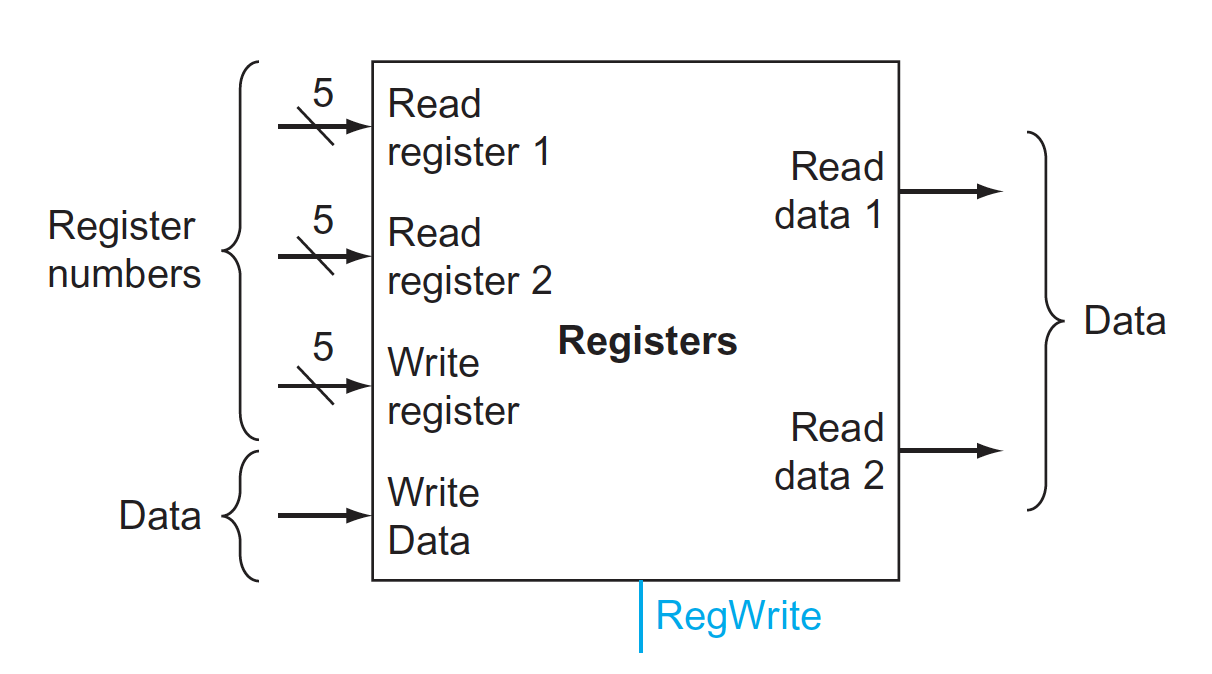
\includegraphics[scale=0.4]{images/register-file.png}
    \end{center}

    Note: the 5 on top of the register number arrows indicate that the register numbers is 5 bits wide, and those bits come from a state element called \emph{instruction memory}, which is where the machine code of our instructions lie.

\end{definition}
\subsection*{R-Type Instructions}
Recall R-format instructions read two registers (\lstinline{rs1} and \lstinline{rs2}), perform an ALU operation on the contents of the registers and write the result to a register (\lstinline{rd}): \lstinline{add rd rs1 rs2}

With that, this means that we need to \emph{read} two data words from the register file and \emph{write} one data word into the register file for each R type instruction.

\textbf{Reading:}\\
For each word to be read from the registers, we need an input to the register file that specifies the \emph{register number} to be read and an output from the register file that will carry the value that has been read from the registers ({\color{red} two outputs? yes.})

\textbf{Writing:}\\
To write a data word, we will need two inputs: one to specify the register number to be written and one to supply the \emph{data} to be written into that register. Writes are controlled by the write control signal, which must be \emph{\textbf{asserted}} for a write to occur at the clock edge.

\subsection*{I Type Instructions}
\subsubsection*{\lstinline{addi}}
Note that for an addi, the output \textbf{Read Data 2} from the register file will a contain garbage value since \textbf{rs2} is not a field of I type instructions, instead it has a 12 bit immediate.

We therefore directly extract the immediate from the instruction memory, and put an arrow directly to the ALU. Moreover, we'd need a unit to \textbf{sign extend} the immediate, call this unit \emph{immediate generator} and a multiplexor to select what will go into the ALU, the Read data 2, or the immediate.

\begin{figure}[h]
    \centering
    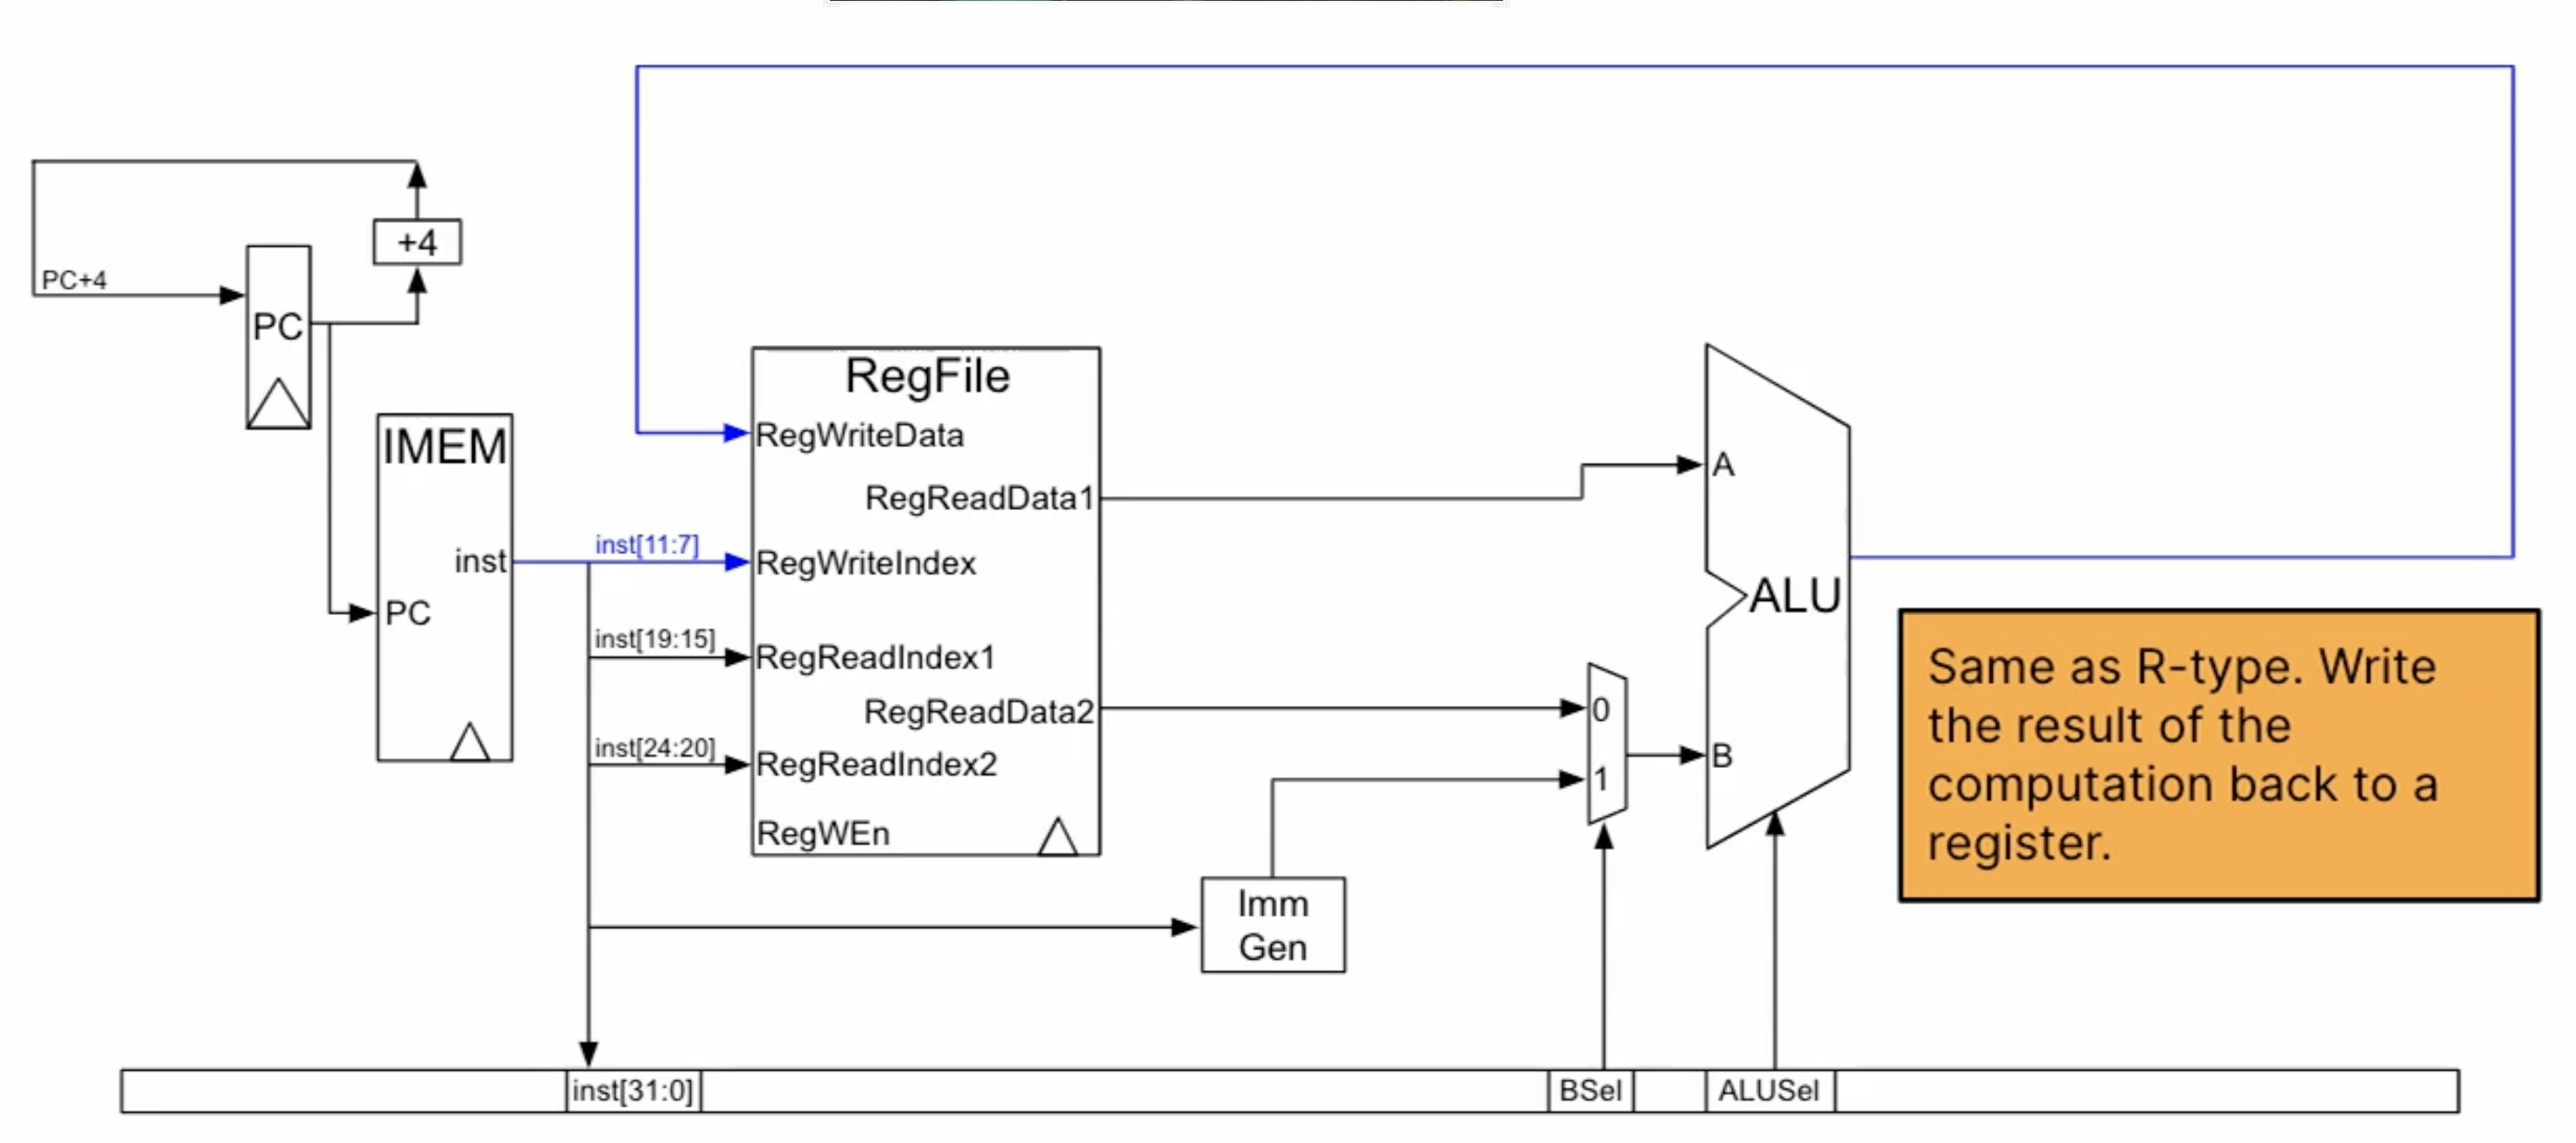
\includegraphics[scale=0.3]{images/addi-datapath.png}
    \caption{Data path for addi instruction.}
\end{figure}

\subsubsection*{Load and Store instructions}
Note a load instruction is a I type instruction with the structure as such:

\lstinline{lw rd imm(rs1)}

where \lstinline{rs1 + imm} is the address we are reading from and we write the value at that address to \lstinline{rd}. And a store instruction is similar except instead of writing to a register, we are writing to memory.

The current data path does not work for load and store instructions, why? Because we don't have a unit for \textbf{data memory} to read from and write to. So lets introduce it.

\begin{figure}[h]
    \centering
    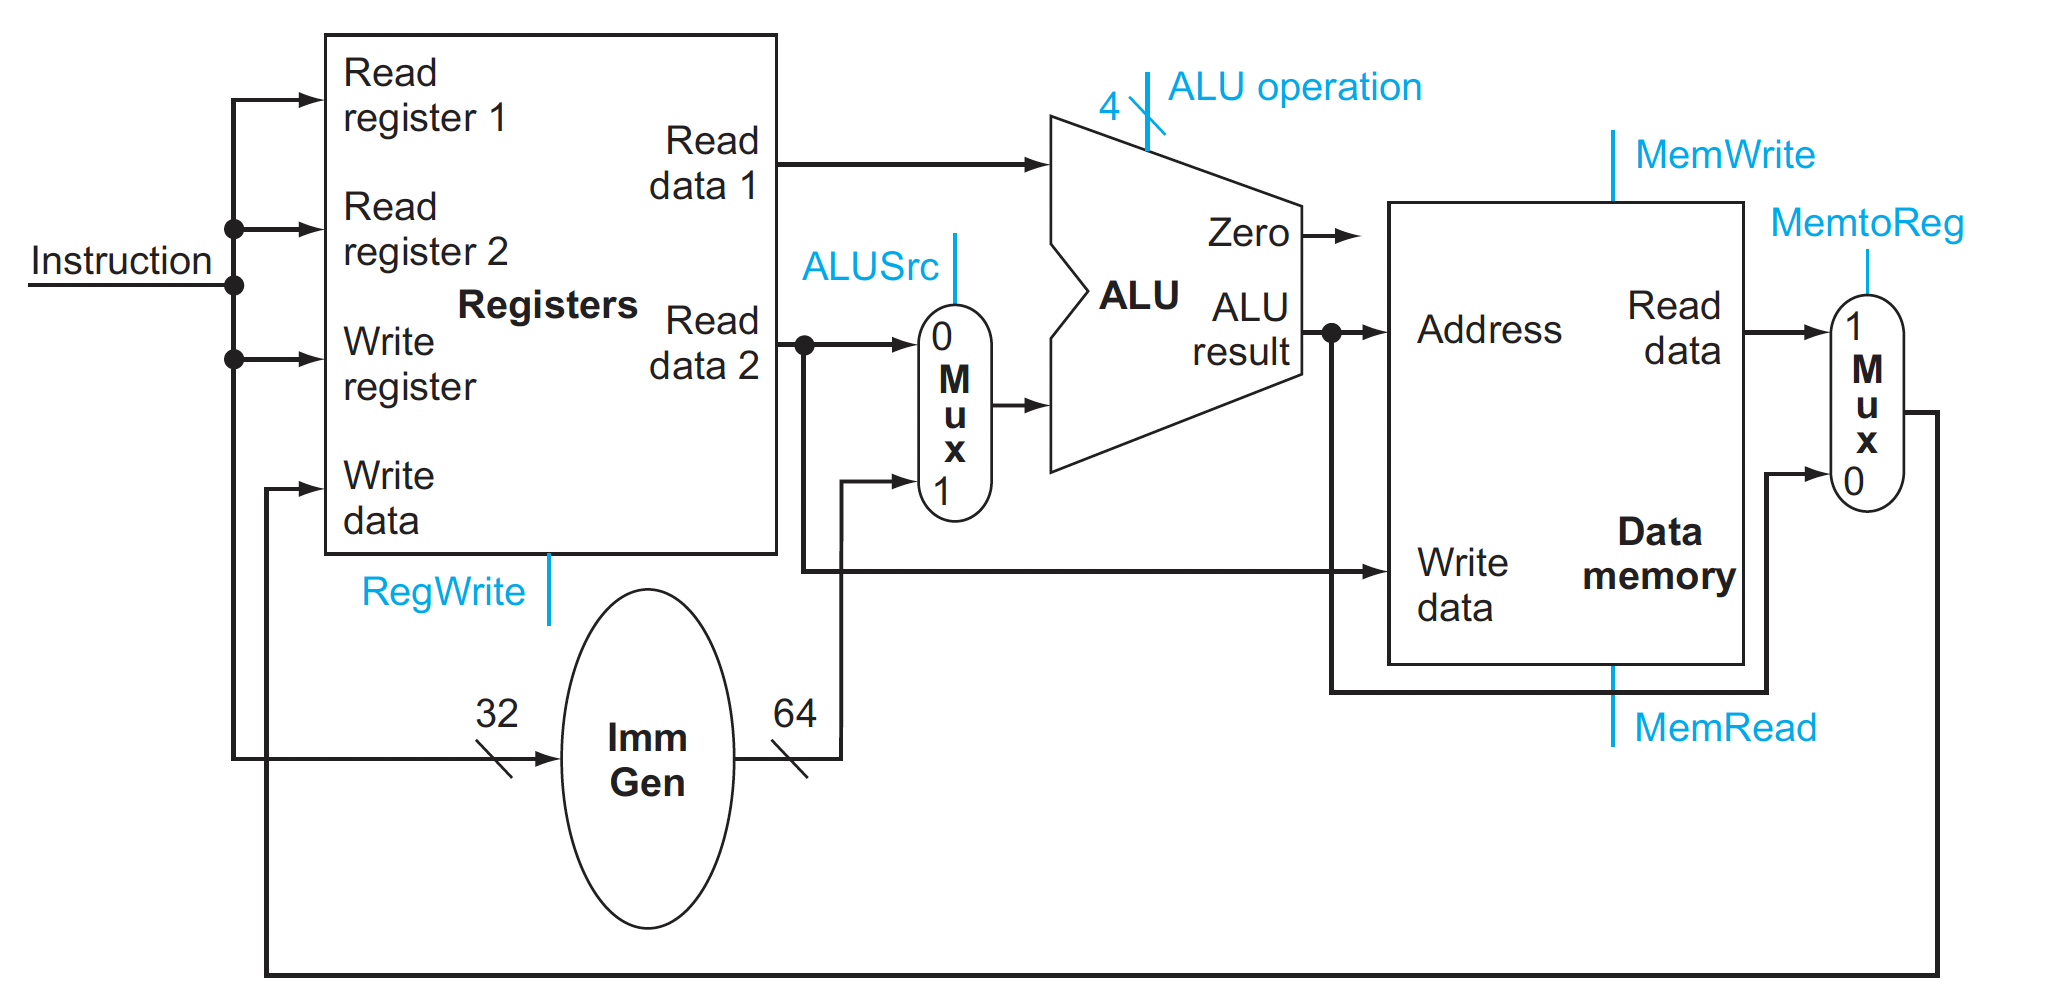
\includegraphics[scale=0.35]{images/memory-instructions-datapath.png}
    \caption{The datapath for memory instructions and the R-type instruction}
\end{figure}
%%%%%%%%%%%%%%%%%%%%%%%%%%%%%%%%%%%%%%%%%%%%%%%%%%%%%%%%%%%%%%%%%
%          Lecture 13: Single Cycle Datapath Controls, Intro to Pipelining
%%%%%%%%%%%%%%%%%%%%%%%%%%%%%%%%%%%%%%%%%%%%%%%%%%%%%%%%%%%%%%%%%
\lecture[07/17/23]{Single Cycle Datapath Controls, Intro to Pipelining}
\subsection*{Pipelining}
\begin{definition}[Pipelining]
    Pipelining is one example of instruction-level parallelism, an implementation technique in which multiple instructions are overlapped in execution.
\end{definition}

Note pipelining does not decrease the time to complete a single instruction, it instead increases instruction  \emph{throughput} since it allows multiple instructions to be processed concurrently, decreasing the total time to complete the work.

\subsubsection*{Pipeline Hazards}
There are situations in pipelining when the next instruction cannot execute in the following clock cycle. These events are called \emph{hazards}, and there are three different types.

\lecture[...]{...}
\lecture[07/20/23]{Parallelism I - Data-Level}

\subsection*{Terminology}
\begin{itemize}
    \item Processors are often called cores in a multicore chip.
    \item SIMD: Single Instruction, Multiple Data. SIMD computers operate on vectors of data. These vectors are specialized vector registers which store 129, 256, or even 512 bits.
    \item For example, a SIMD instruction might add 64 numbers by sending 64 data streams to 64 ALUs to form 64 sums within a single clock cycle.
\end{itemize}

\subsection*{Chapter 6.1: Introduction}
\begin{itemize}
    \item Computer architects seek to create powerful computers by connecting many smaller ones, leading to the concept of multiprocessors.
    \item Multiprocessors can also improve system availability by supporting operation even in the presence of hardware failures.
    \item Multicore microprocessors, which are expected to increase with Moore's Law, are mostly Shared Memory Processors (SMPs) sharing a single address space.
    \item The industry faces the challenge of creating hardware and software that can efficiently execute parallel processing programs with an increasing number of cores.
\end{itemize}

\subsection*{Chapter 6.2: The Difficulty of Creating Parallel Processing Programs}
\begin{itemize}
    \item Creating efficient parallel processing programs has proven to be challenging, particularly as the number of processors increases.
    \item Uniprocessor design techniques, such as instruction-level parallelism, have reduced the need for rewriting programs for multiprocessors.
    \item Efficient parallel programs require breaking tasks into equal-sized pieces, load balancing, and addressing synchronization and communication overhead.
    \item Amdahl's Law reminds us that even small portions of a program must be parallelized to fully utilize many cores.
\end{itemize}

\subsection*{Chapter 6.3: SISD, MIMD, SIMD, SPMD, and Vector}
\begin{itemize}
    \item Parallel hardware can be categorized based on the number of instruction streams and data streams.
    \item SISD (Single Instruction Single Data) refers to conventional uniprocessors with one instruction stream and one data stream.
    \item MIMD (Multiple Instruction Multiple Data) refers to conventional multiprocessors with multiple instruction streams and multiple data streams.
    \item SPMD (Single Program Multiple Data) is a programming style for MIMD computers where a single program runs on all processors.
    \item SIMD (Single Instruction Multiple Data) operates on vectors of data, executing the same instruction simultaneously on multiple data streams.
    \item SIMD's virtues include synchronized execution units and reduced instruction bandwidth.
    \item SIMD works best for data-level parallelism, where arrays are processed in for loops.
    \item SIMD's weakness lies in case or switch statements, leading to reduced performance.
    \item SIMD in x86 architecture includes Multimedia Extensions (MMX), Streaming SIMD Extensions (SSE), and Advanced Vector Extensions (AVX).
    \item Vector architectures, a form of SIMD, involve pipelined execution units and a set of vector registers.
    \item Vector instructions specify a significant amount of work, reducing dynamic instruction bandwidth and control hazards.
    \item Vector architectures are known for their ease in handling data-level parallelism.
    \item Vector instructions accessing memory have a known access pattern, benefiting memory access efficiency.
    \item Vector units are advantageous if the application domain can often use them.
    \item Vector architectures and multimedia extensions differ in the number of operations specified and the handling of data transfers.
    \item Vectors support both strided and indexed accesses for data in memory.
    \item Vector arithmetic instructions usually operate on specific elements of vector registers, facilitating parallelism through multiple vector lanes.
\end{itemize}







%%%%%%%%%%%%%%%%%%%%%%%%%%%%%%%%%%%%%%%%%%%%%%%%%%%%%%%%%%%%%%%%%
%          LECTURE 16: Thread - Level Parallelism
%%%%%%%%%%%%%%%%%%%%%%%%%%%%%%%%%%%%%%%%%%%%%%%%%%%%%%%%%%%%%%%%%
\lecture[07/20/23]{Parallelism II - Thread-level}
\begin{definition}[Hardware Multithreading]
    Increasing utilization of a processor by switching to another thread when one thread is stalled. Hardware multithreading allows multiple threads to share the functional units of a \emph{single} processor in an overlapping fashion to try to utilize the hardware resources efficiently. Note to permit this sharing, the processor must duplicate the independent state of each thread.
\end{definition}

\begin{definition}[Thread]
    A thread includes the program counter, the register state, and the stack. It is a lightweight
\end{definition}

\subsection*{SIMD: Single Instruction, Multiple Data}
\begin{itemize}
    \item Computer applies a single stream to multiple data streams.
    \item Note this will require multiple processing units (1 for each element in the vector) inorder to compute the result of a vector operation.
\end{itemize}

\subsection*{MISD: Multiple Instruction, Single Data}
\begin{itemize}
    \item Computer applies multiple different operations to the same data.
\end{itemize}

\subsection*{MIMD: Multiple Instruction, Multiple Data}
\begin{itemize}
    \item Computer applies multiple different operations to multiple different data.
\end{itemize}

\section*{Parallel Threads}
\begin{definition}[Threads]
    A thread stands for "thread of execution", is a single stream of instructions.
    \begin{itemize}
        \item a program / process can split, or fork itself into separate threads, which can (in theory) execute simultaneously.
    \end{itemize}
    With a single core, a single CPU can execute many threads by \textbf{time sharing.} (note a single core can run one thread at any given time.)

    The CPU is composed of multiple cores, thus allowing multiple threads to be run simultaneously.
\end{definition}
Each core provides one or more hardware threads that actively execute instructions

The \textbf{Operating System} is responsible for managing which threads get run on which CPUs (among other tasks)

\subsection*{Parallel Programming}. In order to create a parallel section: you use \lstinline{#pragma omp parallel ... }

The code in the parallel section gets run on all threads, so we need some way to distinguish threads

Recall that OS chooses which ever thread it wants to run, and can change threads at any time. Therefore a program that uses multithreading is no longer deterministic, i.e. it has random behavior.

A multithreaded program is only considered correct if ANY interlacing of threads yield the same result.

In general with OpenMP, variables declared inside the parallel block will be private to each thread, but variables declared outside a parallel block will be shared across all threads

OpenMP has built-in functionality for dividing up the work of for loops among threads. To tell openMP to split up the work among multiple threads, you would use \lstinline{#pragma omp parallel for}


%%%%%%%%%%%%%%%%%%%%%%%%%%%%%%%%%%%%%%%%%%%%%%%%%%%%%%%%%%%%%%%%%
%          LECTURE 18: Caches
%%%%%%%%%%%%%%%%%%%%%%%%%%%%%%%%%%%%%%%%%%%%%%%%%%%%%%%%%%%%%%%%%
\lecture[...]{...}
\lecture[07/25/23]{Caches I}
Caches – a safe place to store things. \emph{Cache} was the name chosen to represent the level of the memory hierarchy between the processor and main memory.

The simpliest way to assign a location in the cache for each word in memory is to assigned the cache location based on the address of the word in memory. This cache structure is called \textbf{direct mapped}, since each memory location is mapped directly to exactly one location in the cache. Almost all direct-mapped caches use this mapping to the a block:

$$
    \text{(Block address) modulo (Number of blocks in the cache)}
$$

If the cache size (number of blocks in the cache) is a power of 2, then modulo can be computed simply by using the low-order $\log_2\text{(cache size in blocks)}$ bits of the address. For example, an 8 block cache uses the 3 lowest bits ($2^3 = 8$) of the block address to index the blocks.

Note that because multiple memory locations can map to the same cache location, we need a way to know whether the data in the cache corresponds to a requested block/word. We solve this by adding a set of \textbf{tags}.
\begin{definition}[Tag]
    A field in a table used for a memory hierarchy that contains the address information required to identify whether the associated block in the hierarchy corresponds to a requested word. Tags therefore will needs just to contain the upper portion of the address, i.e., the bits not used as an index into the cache.
\end{definition}

We also needs a way to recognize that a cache block does not have valid information. We can't just set the blocks to all zeros at indecies where the cache is not valid since all zeros might actually be a valid entry. Thus, the most common method is to add a separate \textbf{valid bit}.
\begin{definition}[Valid Bit]
    A field in the tables of a memory hierarchy that indicates that the associated block in the hierarchy contains valid data.
\end{definition}
\subsection*{How is the hierarchy managed?}
\begin{enumerate}
    \item Communicaition between Registers $\leftrightarrow$ Memory: By \textbf{compiler} (or assembly level programmer)
    \item Communicaition between Cache $\leftrightarrow$ Main memory: By the \textbf{cache controller hardware}.
    \item Main Memory $\leftrightarrow$ Disks: By the \textbf{OS} (virtual memory)
\end{enumerate}

\subsection*{Locality}
Main idea: predict what emmory might be accessed next based on what memory was already accessed.

The two types of locality are:
\begin{enumerate}
    \item Temporal Locality
          \begin{itemize}
              \item Means: if a memory location is referenced then it will tend to be referenced again soon.
              \item Consequences: keep most recently accessed data items in our cache
          \end{itemize}
    \item Spatial Locality
          \begin{itemize}
              \item Means: if a memory location is references, the locations with nearby addresses will tend to be referenced soon.
              \item Consequences: move blocks consisting of contiguous words instead of just one word at a time.
              \item To faciltate this, we will divide memory into "blocks" of size some power of 2.
              \item Blocks will be assigned  a number, called their tags
          \end{itemize}
\end{enumerate}

\subsection*{Fully Associative Cache}
When a memory access occurs, here are the steps that happen.
\begin{enumerate}
    \item Check if the cache contains the data needed. If so, return the data.
    \item If the data is not present in the cache, load the block of memory into the cache.
    \item Return the data.
\end{enumerate}
A fully associative cache is parameterized on two aspects: the block size, and the number of blocks that can be stored in the cache.

\begin{example}
    \textbf{Lets say we have a cache of 4 byte blocks and 4 blocks of storage. What is the size of the cache?}

    \emph{since the cache stores 4 blocks, and each block is 4 bytes. The size of the cache is 16 bytes}

    \textbf{How do we access address $0x3C1$}

    \emph{we split the address into a tag and offset. Since each block is 4 bytes long, the offset needs to be 2 bits inorder to index into those bytes of data ($2^2 = 4$).}

    $$0x3C1 = 0b\overbrace{{\color{orange}1111 \; 0000}}^{\text{tag}}\underbrace{{\color{blue} 01}}_{\text{offset}}$$

    \emph{after which we scan the tags in the table for matches, and if the valid bit is asserted, then our data is in the cache, so we get the byte at the offset ($0b01 = 1)$}

    \textbf{What if the valid bit was off?}

    \emph{This is called a \textbf{cache miss}. We need to go into main memory and load the block into the cache}


    \textbf{What if there was not tag matches and the cache is already full of valid data?}

    \emph{This is called a \textbf{cache miss with eviction.} There is different eviction policies used for which block we replace, such as LRU, FIFO, or Random}
\end{example}

\lecture[07/26/23]{Caches II: Direct-Mapped and Set Associative Caches}

\subsection*{Direct Mapped Caches}
Note we covered the \textbf{fully-associative cache} in lecture 18. This scheme has certain problems.
\begin{enumerate}
    \item The first problem is, it's hard to find a good and efficient replacement policy.
    \item The second problem is that it requires a lot of comparators/circuitry; a comparator for each block in the table to check for tag equality for all spots.
\end{enumerate}

\begin{center}
    \begin{tabular}{| c c c |}
        \hline
            & Memory Address & \multicolumn{1}{c|}{ }      \\ \hline
        Tag & Index          & \multicolumn{1}{c|}{Offset} \\ \hline
    \end{tabular}
\end{center}

\subsubsection*{Terminology}:
\begin{itemize}
    \item Tag: What's the unique ID.
    \item Index: What row in the table?
    \item Offset: What column/byte? size is determined by "x-bytes per block" which indicates how long each block is.
\end{itemize}


\subsection*{Set Associative Cache}
Set associate caches are similar to direct-mapped caches. A direct mapped is a 1 way set associative cache.
An n way set associative cache is where each index in the table holds N block of data.


\lecture[07/27/23]{Caches III: Performance, Multilevel Caches, Coherence}
\subsection*{Cache Performance Terminology}
\begin{itemize}
    \item \textbf{hit rate:} the percetnage of access that result in a hit.
    \item \textbf{miss rate:} the percentage of access that result in a miss ( 1 - hit rate )
    \item \textbf{hit time:} how long it takes to check the cache + the \textbf{miss penalty}, which is how long it takes to access main memory after a miss.
    \item \textbf{Average Memory Access Time} or (\textbf{AMAT}) is the average amount of time it takes for one memory access, given a program.
\end{itemize}

$$ \text{AMAT} = \text{hit time} + (\text{miss rate} \cdot \text{miss penalty}) $$

\subsection*{Optimizing Cache Hardware}
Benefits of a larger block size:
\begin{itemize}
    \item spatial locality
    \item Reduces comulsory misses6g
    \item works well for programs since a program is run instruction by instruction or sequential array accesses
\end{itemize}

Drawbacks of Larger Block Size
\begin{itemize}
    \item Ping Pong Effect. Imagine a cache with only one very very large
\end{itemize}

\subsection*{Multilevel Caches}
In out current setup, if a cache hits, then we get fast memory access. If a cache miss, then slow access.
If we want to make the cache bigger/more complex, hit rate improves, but also hit time. With just one cache, we need to make some tough trade-offs.

The solution to this is to add \textbf{multiple layers of caches}
/\begin{figure}[h]
    \centering
    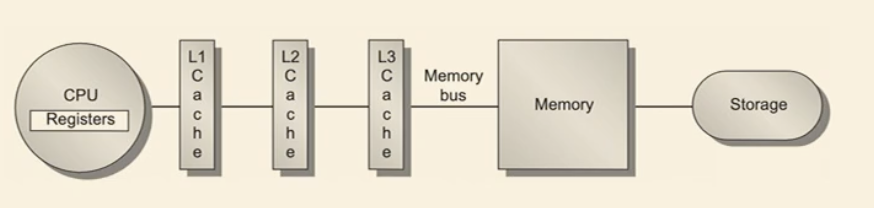
\includegraphics[scale=1.0]{images/multilevelcaches.png}
    \caption{Conceptual Organization of Multilevel Caches}
\end{figure}

Each level of cache is larger than the previous and holds all of the data in the previous cache.

\lecture[07/31/23]{Virtual Memory: I}
\begin{definition}[Virtual Memory]
    a technique that uses main memory as a "cache" for secondary storage.
\end{definition}

\subsection*{Introduction}
\begin{enumerate}
    \item VM ensure protection from other programs.
    \item Gives each process the illusion of a full memory address space that it has completely for itself.
\end{enumerate}

\subsection*{Indirection}
With VM, the processor produces a \textbf{virtual address}, which is translated by a combination of hardware and software to \emph{physical address}, which in turn can be used to access main memory.

In other words, blocks of memory (called \textbf{pages}) are mapped from on address space (called virtual address space) to another address space (called physical address space).

We map a virtual address to a physical address, either to RAM address space (or to the Disk since main memory acts like cache for the disk, i.e., not all the memory is in there.)

\subsection*{Paged Memory}
The concepts at work in virtual memory and in caches are the same, their differing historical roots have lead to the use of different terminology. A virtual memory block is called a \emph{page}, and a virtual memory miss is called a \textbf{page fault}.

Memory is broken into pages and disk access loads an entire page into memory. With this, we can see that memory address are broken into page number (the upper portion of the address), and page offset (lower portion of address)(similar to cache mapping), and that the \textbf{virtual page number is mapped to a physical page number.} Note that the offset is the same for the virtual page and physical page since we map entire virtual pages (offset is relative). So how does this mapping actually work...? Page tables.

\subsection*{Page Tables}
In virtual memory systems, we locate pages by using a table that indexes the memory; this structure is called a \textbf{page table}, and it resides in memory.
\begin{definition}[Page Table]
    The table containing the virtual to physical address translations in a virtual memory system. The table, which is stored in memory, is typically indexed by the virtual page number; each entry in the table contains the physical page number for that virtual page if the page is currently in memory, which is indicated by a valid bit.
\end{definition}

Each program has it's own page table, which maps the virtual address space of that program to main memory. To indicate the location of the page table in memory, the hardware includes a register that points to the start of the page table; we call this the \emph{page table register}
\begin{figure}[H]
    \centering
    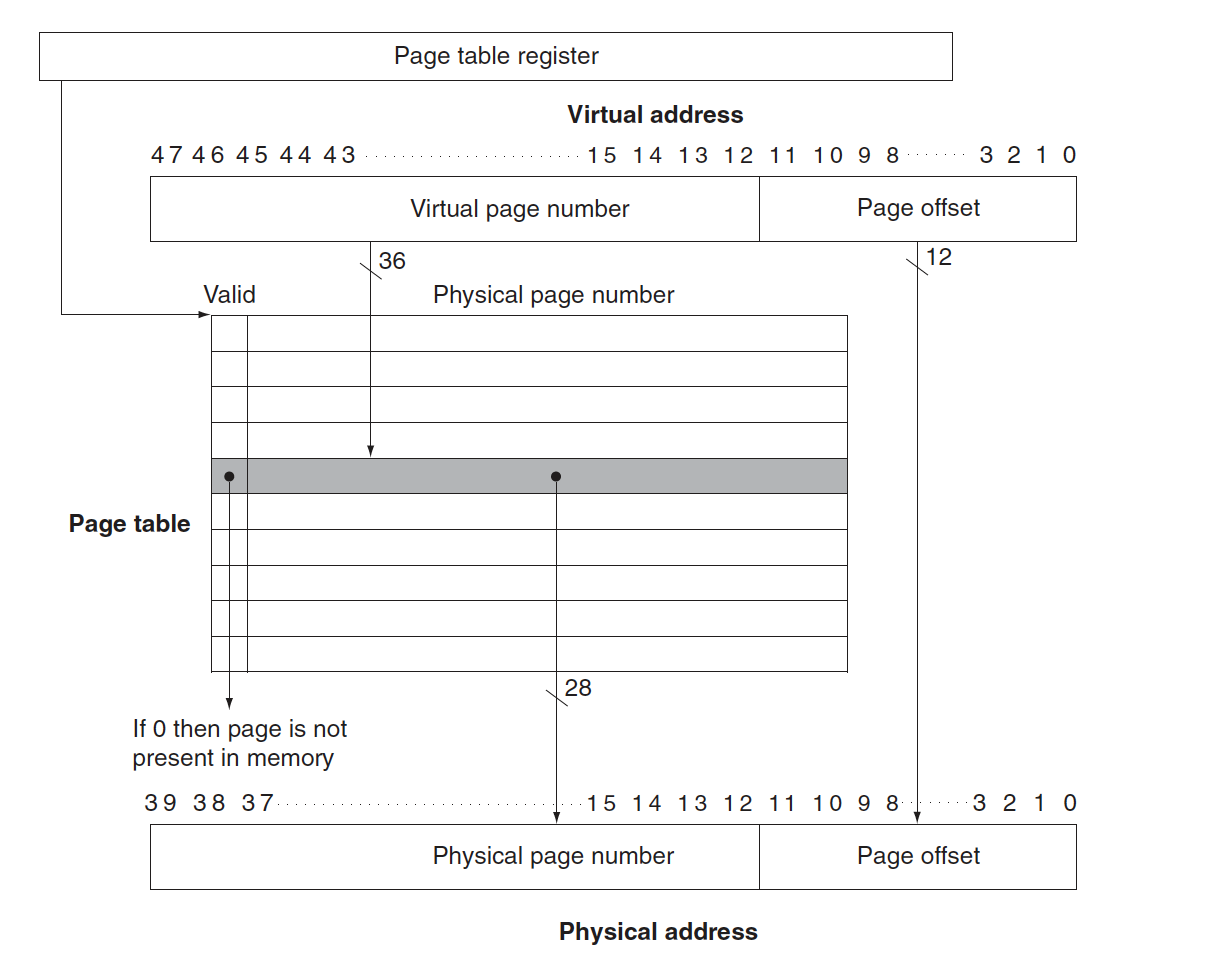
\includegraphics[scale=0.38]{images/page-table.png}
    \caption{Virtual page address mapping to physical page address. We assume a 48-bit address.}
\end{figure}

\subsection*{Page Faults}
If the valid bit for a virtual page is off, a page fault occurs. The operating system must be given control. This transfer is done with the exception mechanism. Once the OS gets control, it must find the page in the next level of the memory hierarchy (usually flash memory or disk) and decide where to place the requested page in main memory.
\end{document}





